\chapter{Introduction}
\section{Problem Background}
The background of this project lies in the requirement for an absolutely robust method of communication with submarines. Due to the nature of how submarines operate, it is considered optimal for messages to be received without having to come to the surface, as this quickly reveals the position which can affect operational effectiveness. 
\\\\
The current solution, in use since the early 20th century uses radio transmissions in the Very Low Frequency band, commonly referred to as long wave. These signals have a range of hundreds of kilometres. Up until the 1960’s the modulation method was a simple on-off keying method, otherwise known as Morse code. In the 1950’s Collins radio developed Minimum Shift Keying (MSK), there is also a variation of MSK called Gaussian Minimum Shift Keying (GMSK) which is where baseband is Gaussian filtered, it is extensively used in mobile phone networks. MSK has been widely adopted in radio communications and used exclusively for communications with submarines since the 1970’s. The advantage of VLF radio is that it can penetrate through several metres of water meaning that a submarine can receive a transmission by towing an aerial underwater. It is also highly resistant to the fallout radiation from a nuclear explosion, unlike other high frequency communications.  
\\\\
MSK is a method of phase modulation. Consider the signal in the complex plane, with a fixed amplitude, rotating with a constant frequency. A signal rotating in the positive direction, anti-clockwise, corresponds to a 1 and rotating in the negative direction, clockwise, corresponds to a zero. The amount of time spent rotating in each direction represents the number of bits in that part of the signal. To extract the message from the signal, the carrier frequency is removed and the phase displacement is calculated.  In a sequence of similar bits, the ideal signal will show a constant phase progression, while the first differential (the instantaneous frequency) will show a consent value. The constant value corresponds to the frequency deviation. When there is a bit change, the sign of the instantaneous frequency will change, causing a crossing of the time axis.

\begin{figure}[h!]
    \centering
    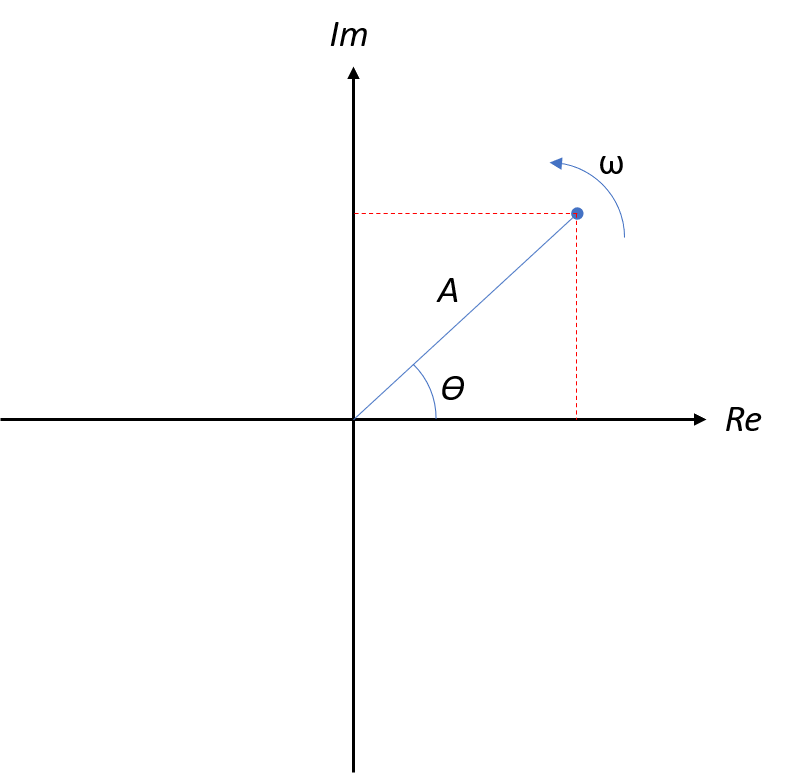
\includegraphics[width = 0.5\textwidth]{figs/phasor.png}
    \caption{Disagram Illustrating Rotating Phasor in the Complex Plane}
    \label{fig:phasor}
\end{figure}

\pagebreak
VLF communications are particularly prone to interference from the broadband electromagnetic radiation created by lightning events leading to symbol loss at the receiver. The electromagnetic interference generated by lightning events is highly impulsive at low frequencies, however at higher frequencies it becomes more Gaussian\footnote{\hyperlink{https://en.wikipedia.org/wiki/Gaussian_noise}{https://en.wikipedia.org/wiki/Gaussian\_noise}}. 
\\\\
Due to the size of transmitters required to broadcast signals with such a low frequency, VLF communications are only one way, shore-to-ship. This means that conventional error correction techniques where the receiver can simply request a re-transmit are simply not possible, the current mitigation strategy for this is that the message is simply rebroadcast many times. Due to the narrow bandwidth of VLF communications the data rate is very low typically around 35 ASCII/UTF-8 characters per second each character having 8 bits. Messages are encrypted before they are modulated into the carrier signal, typically using a one-time pad cipher. This means that the submarine may have to spend a long time close to the surface in order to receiver the message enough times in order to complete it. Here lies the requirement to further investigate these signals to develop a method that can increase the robustness of symbol recovery and estimate wherein the signal symbol loss may have occurred. 

\section{Introduction to the Investigation}
The basis of this problem lies in the recovery of a square-wave/Piecewise signal from a noise corrupted signal. This is a problem that needs to be analysed in the complex plane, by analysing signals as complex sinusoids. There are real world recordings available to analyse, recorded near Bath at a time of particularly high levels of lightning activity
\\\\
The signals from VLF transmitters are readily accessible within broadband low frequency atmospheric recordings, as these transmitters are designed to reach all over the world by utilising the ability of long wave radio to reflect off the ionosphere. They are easily extracted from a broadband recording using a bandpass filter. Through demodulating the passband the original bits can be found, although this may seem too simple given the secretive nature of the communications. The original message is not known however, and herein lies that purpose of the investigation. The ability to improve bit recovery without information contained within the message allows for potential simplification of the communications system.
\\\\
The complex sinusoid can be viewed as having three components:
\begin{enumerate}
    \item \textbf{Transmitter Signal }
    \\
    Directly relates to the complex sinusoid of the frequency modulated carrier.
    \item \textbf{Background Gaussian Noise}
    \\
    This noise is typically low amplitude and can be statistically considered to be normally distributed.
    \item \textbf{Atmospheric Impulsive Noise}
    \\
    This is the result of broadband electromagnetic interference generated by lightning events. Typically described statistically by a long tailed distribution.
\end{enumerate}

This investigation is only really interested in 1 and 3 as Gaussian noise is relatively easy to predict and reduce the impact on message recovery. However, lightning is very powerful and somewhat random which makes it inherently more difficult to mitigate against. The signal from the transmitter remains constant throughout and on top of that during a lightning event there is additive noise within the signal. This pulls the signal away from the plane in which the transmitter is operating and then returns it at another point. As the methods of signal recovery rely on calculating the difference in phase a problem arises.
\\\\
The objective of this investigation is to develop a method of extracting the original symbols from the received signal so that the impact of lightning is mitigated and ideally removed. In order to achieve this a wide variety of literature has been reviewed in order to develop a thorough understanding and an appropriate methodology to tackle the problem. 


